\documentclass[a4paper,12pt]{article}
\usepackage[utf8]{inputenc}
\usepackage[russian]{babel}
\usepackage{amsmath}
\usepackage{graphicx}
\usepackage{hyperref}

\title{\textbf{Документация к проекту "Тетрис"}}
\author{kimikodo}
\date{\today}

\begin{document}

\maketitle

\section{Введение}
Введение в документацию к проекту \("\)Тетрис\("\).

\section{Структура проекта}
Структура проекта \("\)Тетрис\("\) следующая:
\begin{itemize}
\item \texttt{src} - каталог с исходным кодом
\item \texttt{src/include} - каталог с заголовочными файлами
\item \texttt{src/brick\_game} - каталог с реализацией игры
\item \texttt{src/brick\_game/tetris} - каталог с реализацией логики игры
\item \texttt{src/gui} - каталог с реализацией интерфейса
\item \texttt{src/gui/cli} - каталог с реализацией интерфейса командной строки
\item \texttt{test\_tetris} - каталог с тестами
\item \texttt{doc} - каталог с документацией
\end{itemize}

\section{Компиляция проекта}
\item \texttt{make} - сборка проекта \("\)Тетрис\("\).
Установка будет вестись в каталог brick\_game, который будет создан вне папки src


Компиляция проекта \("\)Тетрис\("\) происходит с помощью Makefile. Компиляция производится с помощью следующих шагов:
\begin{itemize}
    \item \texttt{all} - основная цель, собирает и устанавливает проект.
    \item \texttt{clean} - удаляет все объектные файлы, исполняемые файлы и другие временные файлы.
    \item \texttt{install} - устанавливает проект в указанную директорию.
    \item \texttt{uninstall} - удаляет установленный проект.
    \item \texttt{format-check} - проверяет форматирование кода.
    \item \texttt{format} - форматирует код в соответствии с заданными правилами.
    \item \texttt{cppcheck} - проверяет код на ошибки с помощью утилиты cppcheck.
    \item \texttt{valgrind} - запускает тесты с использованием утилиты valgrind.
    \item \texttt{leaks} - проверяет наличие утечек памяти.
    \item \texttt{coverage\_flag} - добавляет флаги для сбора информации о покрытии кода.
    \item \texttt{sanitize} - запускает проект с включенными флагами санитизации.
    \item \texttt{sanitize\_flag} - добавляет флаги санитизации.
    \item \texttt{gcov\_report} - собирает отчет о покрытии кода с помощью утилиты gcovr.
    \item \texttt{test} - запускает тесты проекта.
    \item \texttt{s21\_tetris.a} - собирает статическую библиотеку s21\_tetris.a.
    \item \texttt{debug} - добавляет флаги для сборки в режиме отладки.
    \item \texttt{dist} - создает архив проекта.
\end{itemize}

\section{Интерфейс}
Интерфейс проекта \("\)Тетрис\("\) реализован с помощью библиотеки ncurses. Интерфейс состоит из следующих компонентов:
\begin{itemize}
\item \texttt{StartMenu} - меню, которое отображается при запуске программы
\item \texttt{GameMenu} - интерфейс игры, который отображается, когда пользователь начинает играть
\item \texttt{EndMenu} - интерфейс, который отображается, когда пользователь заканчивает играть
\item \end{itemize}
\section{Логика игры}
Логика игры \("\)Тетрис\("\) реализована с помощью конечного автомата. Конечный автомат имеет следующие состояния:
\begin{itemize}
\item \texttt{NewGame} - состояние, в котором игра ожидает, пока пользователь не нажмет кнопку "Enter"
\item \texttt{SpawnFigure} - состояние, в котором игра генерирует новую фигуру
\item \texttt{Refresh} - состояние, в котором игра отображает фигуру и ожидает, пока пользователь не нажмет кнопку
\item \texttt{Paused} - состояние, в котором игра приостановлена пользователем
\item \texttt{SureEndGame} - состояние, в котором игра выводит окно с подтверждением выхода из игры.
Нужно для предотвращения случайного нажатия
\item \item \texttt{EndGame} - состояние, в котором игра заканчивается
\end{itemize}
\begin{figure}[h]
\center{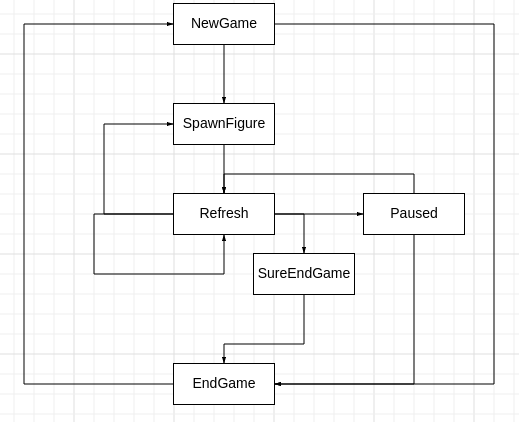
\includegraphics[width=0.6\linewidth]{FinitMachine.png}}
\caption{Конечный автомат}\label{fig:FinitMachine}
\end{figure}

\begin{figure}[h]
    \center{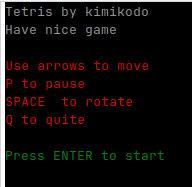
\includegraphics[width=0.6\linewidth]{StartMenu.png}}
    \caption{Начальный интерфейс}\label{fig:StartMenu}
\end{figure}
\begin{figure}[h]
    \center{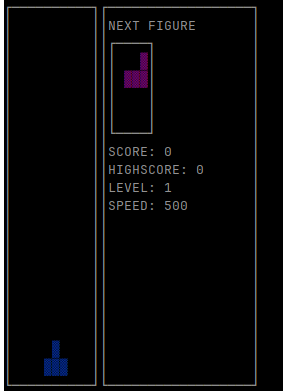
\includegraphics[width=0.6\linewidth]{GameMenu.png}}
    \caption{Интерфейс игры}\label{fig:GameMenu}
\end{figure}
\begin{figure}[h]
    \center{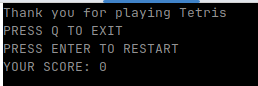
\includegraphics[width=0.6\linewidth]{EndMenu.png}}
    \caption{Завершающий интефейс}\label{fig:EndMenu}
\end{figure}
\end{document}